%%% Содержимое слайдов

\frame[plain]{\titlepage} % Титульный слайд

%-------------------------------------------------------------------------------

\section{Разработка виртуальной инфраструктуры для реализации облачных услуг}

\begin{frame}
\frametitle{\insertsection}
Требования:
\begin{itemize}
	\item устранение единых точек отказа
	\item защита от несанкционированного доступа и DDoS-атак
	\item \textbf{использование свободного ПО}
	\item документирование инфраструктуры
	\item автоматизация инфраструктуры
	\item разработка эффективных тарифных планов хостинга
\end{itemize}
\end{frame}

%-------------------------------------------------------------------------------

\section{Общая схема инфраструктуры}

\begin{frame}
\frametitle{\insertsection}
\begin{figure}[h]
	\center
	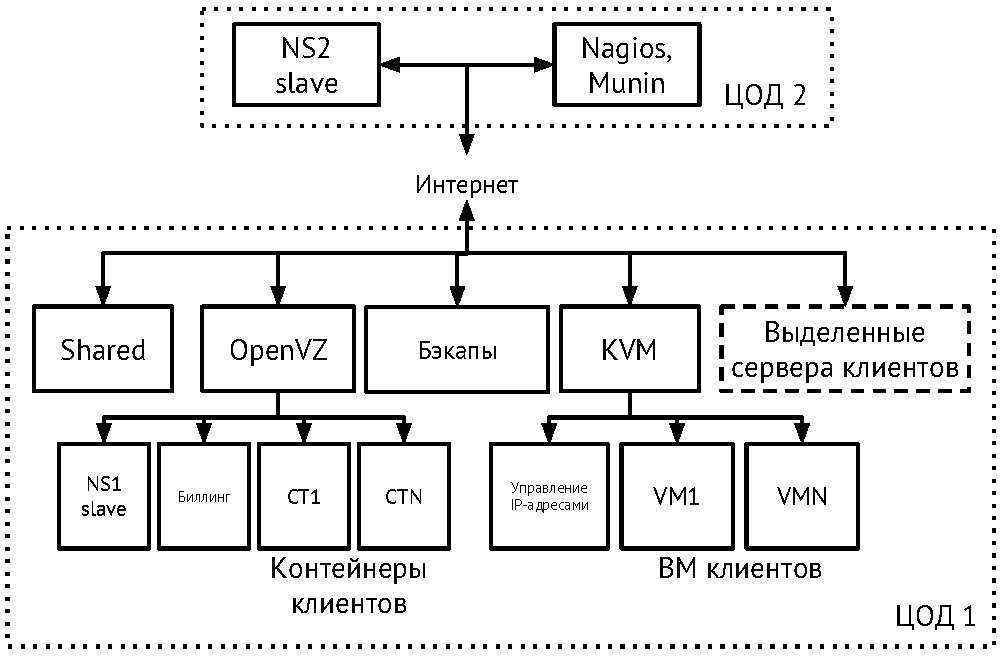
\includegraphics[width=\linewidth]{infrast-scheme}
\end{figure}
\end{frame}

%-------------------------------------------------------------------------------

\section{Серверная операционная система}

\begin{frame}
\frametitle{\insertsection}
\framesubtitle{CentOS 7 (GPL)}
Преимущества:
\begin{itemize}
	\item 494 из 500 крупнейших суперкомпьютеров работают на Linux
	\item поддержка 6-10 лет
	\item свободно распространяемая ОС
	\item большое количество документации
	\item имеется опыт работы с дистрибутивом
\end{itemize}
\end{frame}

%-------------------------------------------------------------------------------

\section{Мониторинг}

\begin{frame}
\frametitle{\insertsection}
\framesubtitle{Nagios\uncover<2->{ > Icinga2 (GPLv2)}}
\begin{figure}[h]
	\center
	\begin{multicols}{2}
		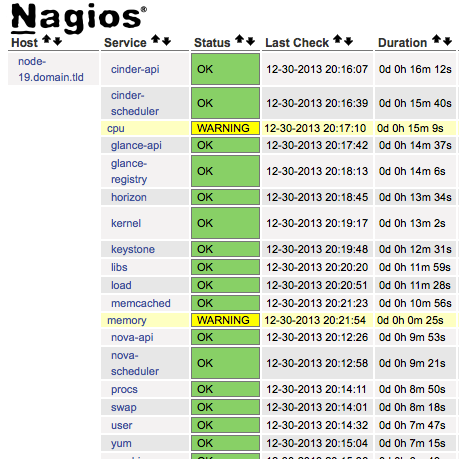
\includegraphics[width=\linewidth]{nagios} \pause \\
		\uncover<2->{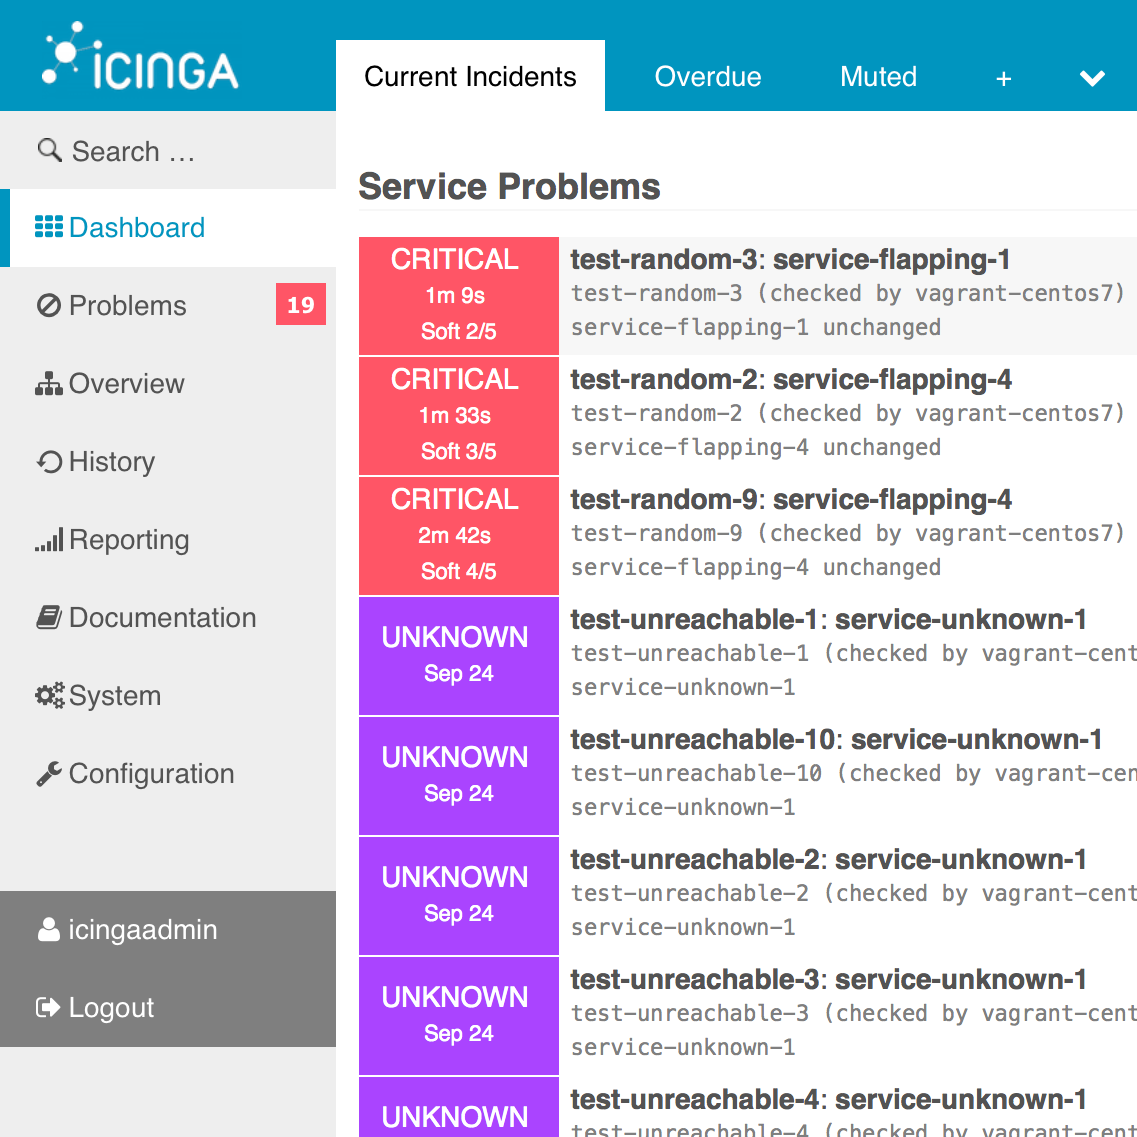
\includegraphics[width=\linewidth]{icinga2}}
	\end{multicols}
\end{figure}
\end{frame}

%-------------------------------------------------------------------------------

\section{Метрики}

\begin{frame}
\frametitle{\insertsection}
\framesubtitle{Munin (GPL)}
\begin{figure}[h]
	\center
	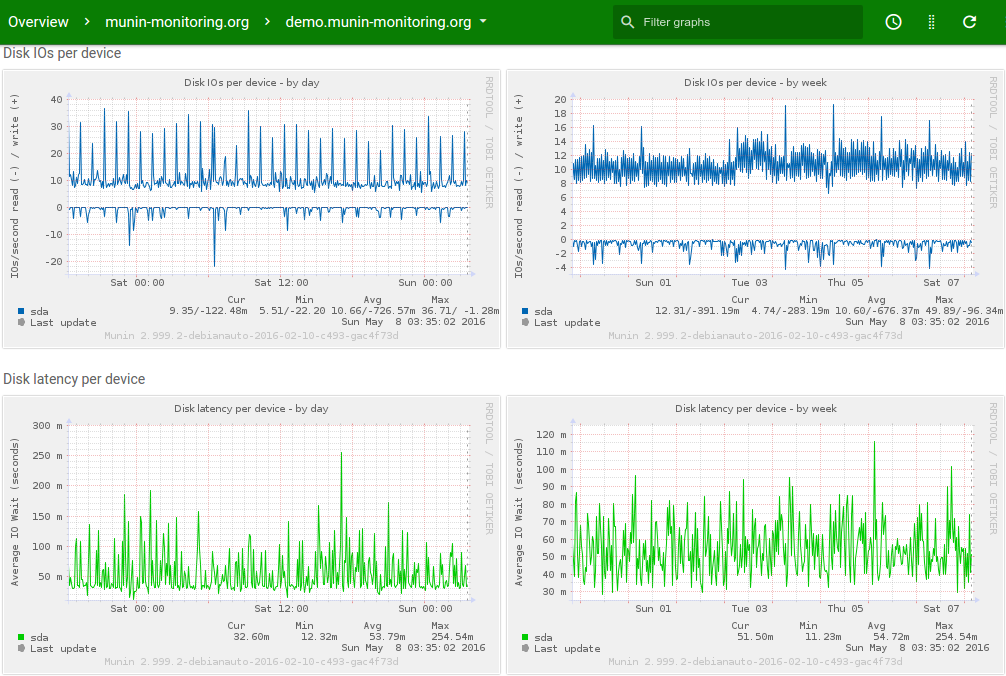
\includegraphics[width=\linewidth]{munin}
\end{figure}
\end{frame}

%-------------------------------------------------------------------------------

\section{Автоматизация управления}

\begin{frame}
\frametitle{\insertsection}
\framesubtitle{Ansible (GPL)}
\begin{figure}[h]
	\center
	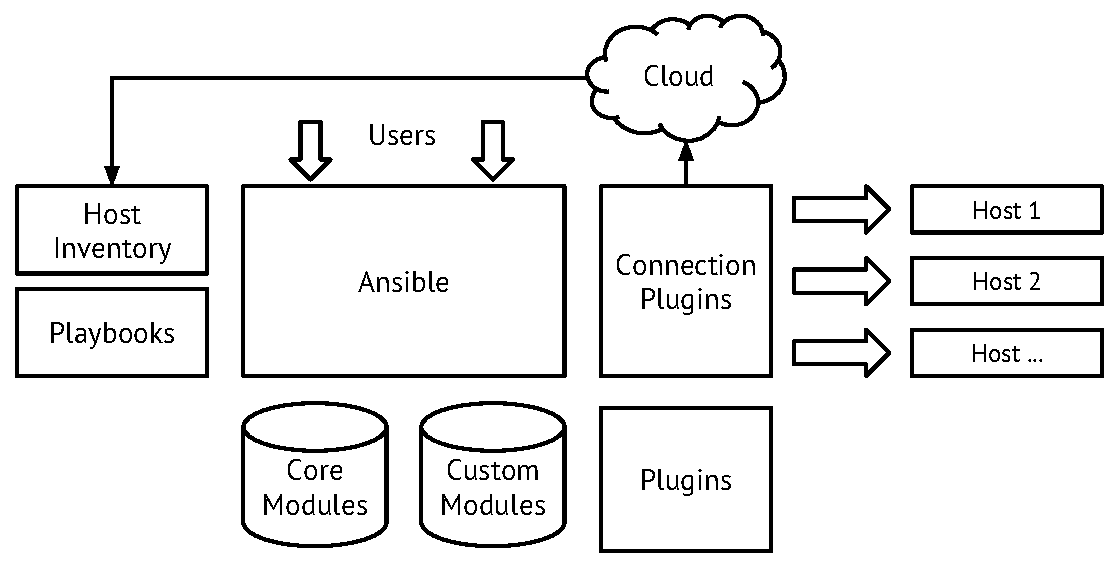
\includegraphics[width=\linewidth]{ansible}
\end{figure}
\end{frame}

%-------------------------------------------------------------------------------

\section{Виртуализация}

\begin{frame}
\frametitle{\insertsection}
\framesubtitle{OpenVZ (GPLv2)\uncover<2->{ + KVM (GPL/LGPL)}}
\begin{figure}[h]
	\center
	\begin{multicols}{2}
		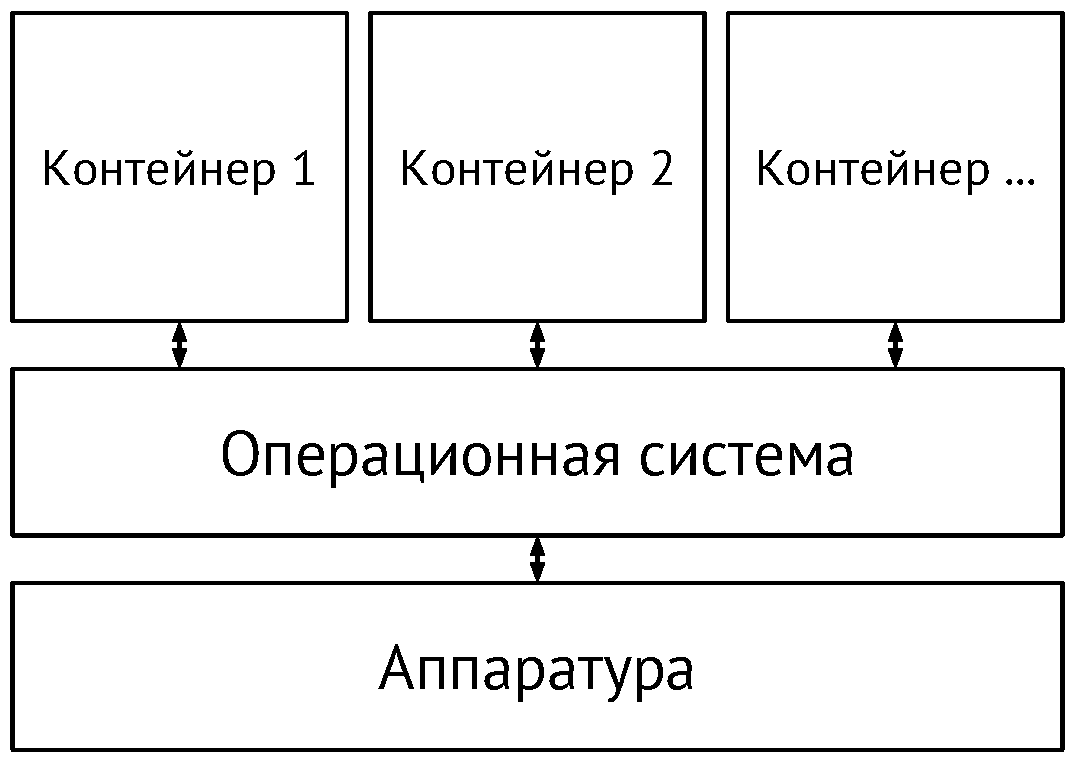
\includegraphics[width=\linewidth]{cont-virt} \\
		OpenVZ \pause \\
		\uncover<2->{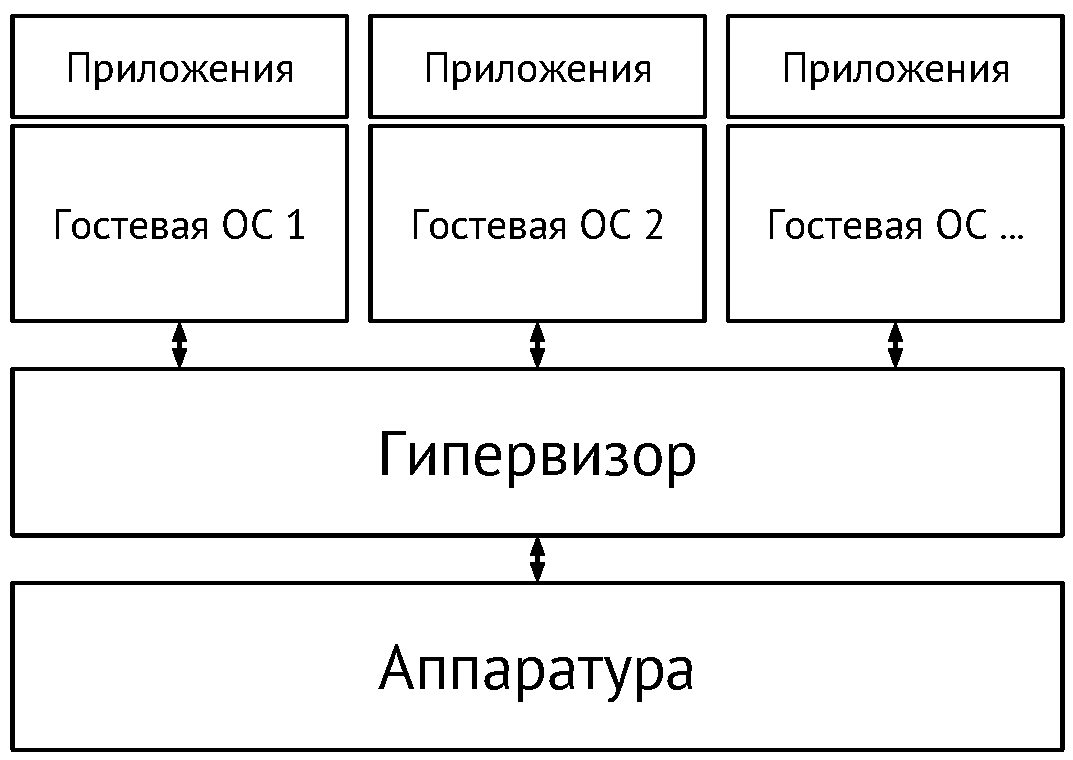
\includegraphics[width=\linewidth]{full-virt}}
		KVM
	\end{multicols}
\end{figure}
\end{frame}

%-------------------------------------------------------------------------------

\section{Стек ПО для виртуального хостинга}

\begin{frame}
\frametitle{\insertsection}
\framesubtitle{LAMP+Nginx, Exim+Dovecot+SpamAssassin+Roundcube (GPL/LGPL/MIT/Apache)}
\begin{figure}[h]
	\center
	\begin{multicols}{2}
		
\includegraphics[width=\linewidth]{lamp} \\
		
\includegraphics[width=\linewidth]{mail}
	\end{multicols}
\end{figure}
\end{frame}

%-------------------------------------------------------------------------------

\section{Защита от вредоносов}

\begin{frame}
\frametitle{\insertsection}
\framesubtitle{Linux Malware Detect (GPL)}
Возможности:
\begin{itemize}
	\item обнаружение вредоносов по хэш-сумме MD5
	\item отправка потенциально опасных файлов на сервис rfxn.com для внесения в базу сигнатур
	\item использование exclude-файлов
	\item удаление инфицированных base64 и gzinflate вставок
	\item перемещение зараженных файлов в карантин
	\item поиск по сигнатурам ClamAV
\end{itemize}
\end{frame}

%-------------------------------------------------------------------------------

\section{Защита сети}

\begin{frame}
\frametitle{\insertsection}
\framesubtitle{ddos-deflate (Artistic License) + IPTables/fail2ban/ipset (GPL)}
\begin{figure}[h]
	\center
	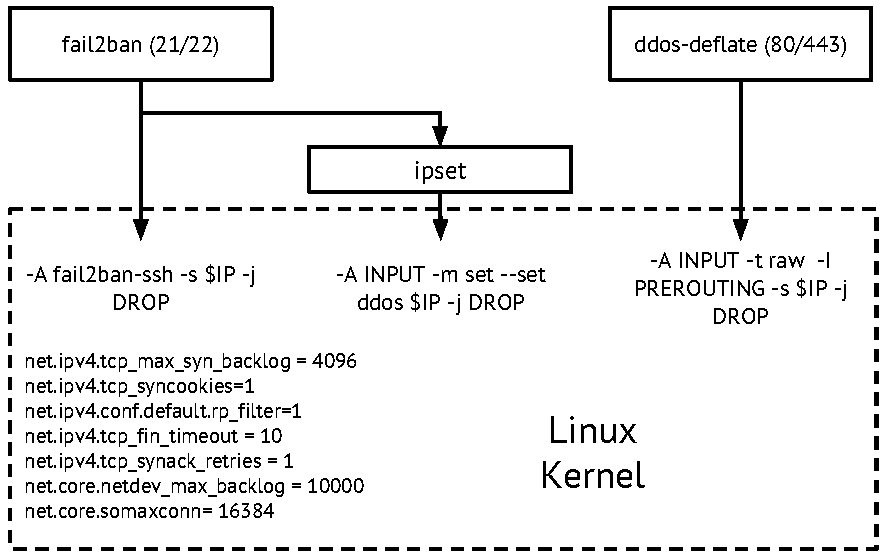
\includegraphics[width=\linewidth]{iptables}
\end{figure}
\end{frame}

%-------------------------------------------------------------------------------

\section{Панели управления для клиентов}

\begin{frame}
\frametitle{\insertsection}
\framesubtitle{Vesta Control Panel (GPLv3)}
\begin{figure}[h]
	\center
	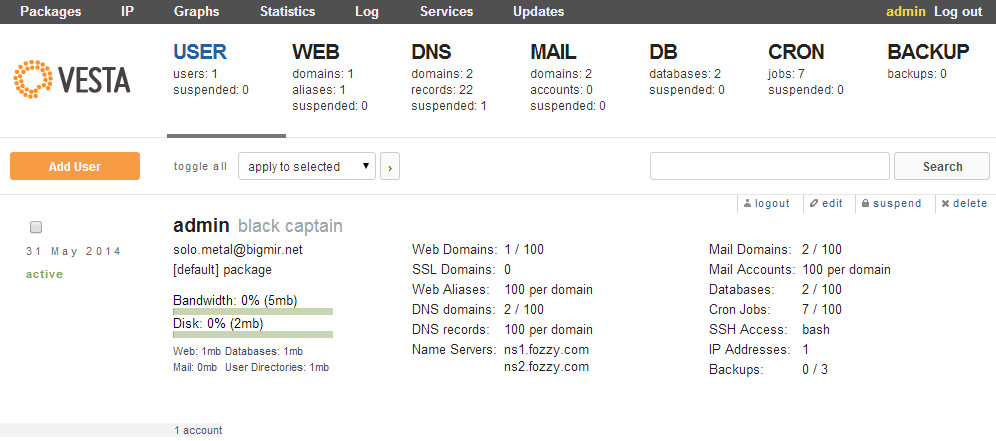
\includegraphics[width=\linewidth]{vesta}
\end{figure}
\end{frame}

%-------------------------------------------------------------------------------

\section{Сравнение с закрытыми аналогами}

\begin{frame}
\frametitle{\insertsection}
\framesubtitle{Стоимость лицензий и обслуживания}
\begin{figure}[h]
	\begin{tabular}{|l|l|}
		\hline
		\bf{Open Source} & \bf{Closed Source} \\ \hline
		CentOS 7 & RHEL 7 --- \$900/год за 1 сервер \\ \hline
		Nagios & Sensu --- \$600/год за 50 серверов \\
		Munin & Opsview --- \$935/год за 50 серверов \\ \hline
		OpenVZ & Virtuozzo --- \$6200/год за 100 контейнеров \\
		KVM & vCenter Server --- \$1750/год за 1 CPU \\ \hline
		Maldet & Virusdie --- \$20/год + \$2/год за сайт \\ \hline
	\end{tabular}
\end{figure}
\begin{itemize}
	\item RHEL 7 (10 серверов) --- \$9 000/год
	\item Virtuozzo (100 контейнеров x 10 серверов) --- \$62 000/год
	\item vSphere Server (4 CPU x 10 серверов) --- \$70 000/год
	\item Sensu/Opsview (30-50 серверов) --- \$600-935/год
	\item Virusdie (2000 сайтов x 10 серверов) --- \$40 000/год
\end{itemize}
Итого: \bf{\$262 600/год}
\end{frame}

%-------------------------------------------------------------------------------

\section{Проекты в Open Source}

\begin{frame}
\frametitle{\insertsection}
\begin{itemize}
	\item openvz-tutorial (CC BY-SA 4.0): \href{https://github.com/Amet13/openvz-tutorial}{github.com/Amet13/openvz-tutorial}
	\item virtuozzo-tutorial (CC BY-SA 4.0): \href{https://github.com/Amet13/virtuozzo-tutorial}{github.com/Amet13/virtuozzo-tutorial}
	\item ddos-defalte (Artistic License 2.0): \href{https://github.com/Amet13/ddos-deflate}{github.com/Amet13/ddos-deflate}
	\item ansible-vz-wordpress (GNU GPLv3): \href{https://github.com/Amet13/ansible-vz-wordpress}{github.com/Amet13/ansible-vz-wordpress}
	\item icinga2-plugins-extra (GNU GPLv3): \href{https://github.com/Amet13/icinga2-plugins-extra}{github.com/Amet13/icinga2-plugins-extra}
	\item \bf{bachelor-diploma (CC BY-SA 4.0)}: \href{https://github.com/Amet13/bachelor-diploma}{github.com/Amet13/bachelor-diploma}
\end{itemize}
\end{frame}

%-------------------------------------------------------------------------------
